\chapter{The Advection Equation}\label{ch:advection-equation}

We now consider differential equations with one dependent and two or
three independent variables, that is, partial differential equations.
More specifically, we shall consider various simplified forms of the
advection equation, describing advection of a dependent variable. This
is considered in practice to be the most important part of the
atmospheric governing equations.

We have already discussed the one-dimensional linear advection equation
to some extent in the introductory chapter. We shall organize the
analysis here so as first to continue considering problems associated
with the simplest one-dimensional linear form of the advection equation,
and then to proceed to problems introduced by more complex forms of the
advection equation.

\section{Schemes with centered second-order space differencing}\label{sec:schemes-centered-second-order-space-diff}

We shall first consider the equation

 \[\frac{\partial u}{\partial t}  +c\frac{\partial u}{\partial x} = 0\]\[c = const.\]

Here \(u = u\left( x,t \right)\) is a function of two independent
variables : the independent variable \(x\) will represent a space
variable, and, thus, \texttt{a1.1} will be called the one-dimensional
linear advection equation. As seen earlier, its general solution is

 \[u = f\left( x - ct \right)\]

where \(f\) is an arbitrary function. The name \emph{advection equation}
was suggested by Phillips (1960).

One of the finite difference schemes for \texttt{a1.1} is the forward
and upstream scheme, which has been shown excessively damping in the
Chapter \texttt{Chapter1} .

If the space derivative in \texttt{a1.1} is approximated by a centered
finite difference quotient using values at the two nearest points, we
obtain for the time derivative

 \[\frac{\partial u_{j}}{\partial t} = - c\frac{u_{j + 1} - u_{j - 1}}{2\Delta x}\]

The subscript here, as before, denotes the distance from the origin in
space increments; that is, \(x = j\Delta x\). A number of schemes for
the numerical solution of \texttt{a1.1} can now be constructed because
we can approximate the time derivative in \texttt{a1.3} by one of the
methods studied in the preceding chapter. For example, when the time
derivative is approximated using the leapfrog scheme, we obtain

 \[\frac{u_{j}^{n + 1} - u_{j}^{n - 1}}{2\Delta t} = - c\frac{u_{j + 1}^n - u_{j - 1}^n}{2\Delta x}\]

as one of many possible consistent schemes for the numerical solution of
\texttt{a1.1}.

The properties of schemes constructed in this way can be inferred from
the known properties of time differencing schemes applied to the
oscillation equation. To see this, we substitute into \texttt{a1.3} a
tentative solution in form of the single harmonic component

 \[u_{j} = Re\left\lbrack U\left( t \right)e^{ikj\Delta x} \right\rbrack\]

After some rearrangement, this gives

 \[\frac{\text{dU}}{\text{dt}} = i\left( - \frac{c}{\Delta t}\sin{k\Delta x} \right)U\]

If we denote

 \[\omega \equiv - \frac{C}{\Delta x}\sin{k\Delta x}\]

this is equivalent to the oscillation equation of the previous chapter.
Now, if we approximate \texttt{a1.6} using one of the time differencing
schemes studied in that chapter, the same finite difference equation is
obtained as when we apply that scheme to \texttt{a1.3} and then
substitute the wave solution \texttt{a1.5}. Hence, properties of finite
difference schemes derived from \texttt{a1.3} can be inferred from the
results of Section \texttt{Section2.1}, where the frequency to is given
by \texttt{a1.7}.

As an example, if \texttt{a1.6} is approximated using the leapfrog
scheme, we obtain

 \[U^{\left( n + 1 \right)} = U^{\left( n - 1 \right)} + 2\left( - c\frac{\Delta t}{\Delta x}\sin{k\Delta x} \right)U^{\left( n \right)}\]

Using the notation of chapter \texttt{Chapter2}, we write

 \[p = - c\frac{\Delta t}{\Delta x}\sin{k\Delta x}\]

We obtain the same finite difference equation \texttt{a1.8} by first
applying the leapfrog scheme to \texttt{a1.3} giving \texttt{a1.4} and
then substituting \texttt{a1.5} into \texttt{a1.4}. Thus, properties of
\texttt{a1.4} can be inferred from (1.7) and from the known properties
of the leapfrog scheme applied to the oscillation equation.

Let us look at some of conclusions obtained in this way. For stability
of the leapfrog scheme it was required that the condition
\( \left| p \right| \leq 1 \) be satisfied for all values of \(\omega\)
occuring. Thus, we have to satisfy

\[\left| c\frac{\Delta t}{\Delta x}\sin{k\Delta x } \right| \leq 1\]

for any admissible k. Since \(\left| \sin{k\Delta x} \right|\) does
reach the maximum value of unity in the admissible range of k, we obtain
the stability condition

 \[\left| c \right|\frac{\Delta t}{\Delta x} \leq 1\]

This criterion, obtained already in the Chapter \texttt{Chapter1}, shows
that stability cannot simply be achieved by reduction of the time and
space increments. Rather, it is necessary to reduce the ratio of these
increments \(\frac{\Delta x}{\Delta t }\) to obtain stability. The
condition \texttt{a1.10} was first found by Courant, Friedrichs and Lewy
(1928), and, therefore, is usually referred to as the
Courant-Friedrichs-Lewy, or CFL, stability criterion.

It is instructive to note that the maximum value of
\(\left| p \right|\), that is, the minimum stability, is associated with
the wave with \(k\Delta x = \frac{\pi}{2}\). This is the component with
wave length 4 \(\Delta x\), twice the shortest resolvable wave length
\(2\Delta x\).

We can also use other results of the previous analysis. There are two
solutions for \(U^{\left( n \right)}\), the physical and the
computational mode

 \[U_{1}^{\left( n \right)} = \lambda_{1}^{n}U_{1}^{\left( 0 \right)}U_{2}^{\left( n \right)}
= \lambda_{2}^{\left( n \right)}U_{2}^{\left( 0 \right)}\]

\(\lambda_{1}\) and \(\lambda_{2 }\) are given here by Eqs.
\texttt{h2.34} of Chapter \texttt{Chapter2}. In the stable case, we
have, for \(p \gtrless 0\)

 \[\lambda_{1} = c^{i\theta}, \qquad \theta = arctan\left( \frac{p}{\sqrt{1 - p^{2}}} \right)\]

\[\lambda_{1} = e^{i\left( \pm\pi-\theta\right)} = - e^{- i\theta}\]

Using \texttt{a1.5}, it is seen that the approximation u{]} also has a
physical and a computational mode. For the physical mode

 \[u_{j}^{n} = Re\left\lbrack U_{1}^{\left( 0 \right)}e^{\left( j\Delta x
+ \frac{\theta}{k\Delta t}n\Delta t \right)} \right\rbrack\]

For the computational mode, on the other hand, we obtain

 \[u_{j}^{n} = Re\left\lbrack \left( - 1 \right)^{n}U_{2}^{\left( 0 \right)}
e^{\text{ik}\left( j\Delta x - \frac{\theta}{k\Delta t} \right)} \right\rbrack\]

These expression can be compared with the true solution of \texttt{a1.1}
in the form of a single harmonic component, as given in chapter
\texttt{Chapter1},

 \[u\left( x,t \right) = Re\left\lbrack U\left( 0 \right)e^{\text{ik}
\left( x - c t \right)} \right\rbrack\]

We find that the phase speed of the physical mode, \(c_{1}\) is equal to
\(- \frac{\theta}{k\Delta t}\), and the phase speed of the
computational mode, \(c_{2}\), considering the even time steps only, is
equal to \(\frac{\theta}{k\Delta t}\) \texttt{a1.12} shows that as
\(\Delta t \rightarrow 0, \quad \theta \rightarrow p\) and \texttt{a1.9}
shows that as
\(\Delta x \rightarrow 0, \quad p  \rightarrow \text{ck}\Delta t\).
Thus, as \(\Delta x,\Delta t \rightarrow 0, \quad c_{1} \rightarrow c\),
that is, the phase speed of the physical mode approaches the phase speed
of the true solution, while at the same time \(c_{2} \rightarrow - c\).
In addition, the computational mode changes sign at all grid points
from time step to time step, because of the factor
\(\left( - 1 \right)^{n}\) in \texttt{a1.14}.

Now let us use another scheme from chapter \texttt{Chapter2} to
approximate the time derivative in \texttt{a1.3}, the Matsuno scheme.
First the approximate values \(u_{j}^{\left( n + 1 \right)^{*}}\) using
the forward scheme, that is,

 \[\frac{u_{j}^{\left( n + 1 \right)^{*}} - u_{j}^{n}}{\Delta t}
= - c\frac{u_{j + 1}^{n} - u_{j - 1}^{n}}{2\Delta x}\]

Then, these approximate values are used in the backward scheme, that is

 \[\frac{u_{j}^{n + 1} - u_{j}^{n}}{\Delta t} =
- c\frac{u_{j + 1}^{\left( n + 1 \right)^{*}} - u_{j - 1}^{\left( n + 1 \right)^{*}}}{2\Delta x}\]

It is instructive to eliminate the approximate values
\(u^{\left( n + 1 \right)^{*}}\) from this equation, by substituting
values given by \texttt{a1.16}, with the subscript \(j\) replaced by
\(j + 1\) and then by \( j - 1\). In this way we obtain

 \[\frac{u_{j}^{n + 1} - u_{j}^{n}}{\Delta t} =
- c\frac{u_{j + 1}^{n} - u_{j - 1}^{n}}{2\Delta x} +
c^{2}\Delta t\frac{u_{j + 2}^{n} -
  {2u}_{j}^{n} + u_{j - 2}^{n}}{\left( 2\Delta x \right)^{2}}\]

Without the last term, this represents the finite difference equation
obtained when the forward scheme is used for the time derivative in
\texttt{a1.3}. The third term approaches zero as
\(\Delta x,\Delta t \rightarrow 0\), and \texttt{a1.18} is therefore
also a consistent scheme for the advection equation. On the other hand,
for a fixed \(\Delta t\) this term approaches
\(c^{2}\Delta t\left( \frac{\partial^{2}u}{\partial x^{2}} \right)\) as
\(\Delta x \rightarrow 0\). It is therefore of the same form as a finite
difference approximation to a Fick\textquotesingle s diffusion term,

and it has a damping effect. This damping effect, however, is dependent
on the wave length. As the third term is calculated over an interval of
\(4\Delta x\), the maximum damping occurs for a wave with wave length of
\(4\Delta x\). There is no damping of the shortest resolvable wave with
wave length \(2\Delta x\). Even if a damping effect were desirable when
solving the advection equation, we would not want this particular
dependence on wave length. Thus, the Matsuno scheme does not appear
suitable for solving the advection equation.

It is convenient to include here one more example of the use of the
energy method for testing stability. In addition to being applicable
also to nonlinear equations, it can be used to study the effect of
boundary conditions on stability. We will use the energy method here to
test the stability of a group of schemes that can be used for solving
\texttt{a1.3}.

A fairly wide class of schemes for solving \texttt{a1.3} can be written
as

 \[u_{j}^{n + 1} - u_{j}^{n} = - \frac{1}{2}\mu\left( {u^{*}}_{j + 1} - {u^{*}}_{j - 1} \right)\]

where

 \[\mu \equiv \frac{c\Delta t}{\Delta x}\]

\begin{description}
 \item[and \({u^{*}}_{j}\) is a linear function of a number of values]
 \(u_{j}^{n}\)
\end{description}

For example, to obtain the non-iterative two level schemes we write

 \[{u^{*}}_{j} = \alpha u_{j}^{n} + \beta u_{j}^{n + 1}\]

For the interative two level shemes write

 \[{u^{*}}_{j} = u_{j}^{n} - \frac{\beta}{2}\mu\left( u_{j + 1}^{n} - u_{j - 1}^{n} \right)\]

Finally, for the Adams-Bashforthsheme

 \[{u^{*}}_{j} = \frac{3}{2}u_{j}^{n} - \frac{1}{2}u_{j}^{n - 1}\]

Here we shall analyze the stability of the non-iterative two level
schemes. It is convenient first to multiply (1.19) by \(u_{j}\) and sum
for all \(j\); we obtain

\[\sum_{j}{u^{*}}_{j}\left( u_{j}^{n + 1} - u_{j}^{n} \right) = - \frac{1}{2}\mu\sum_{j}u^{*}_{j}\left( u^{*}_{j+1} - u^{*}_{j - 1} \right)\]

The right hand side vanished if cycle boundary conditions are assumed ;
we then have

\[\sum_{j}u^{*}_{j}\left( u_{j}^{n + 1} - u_{j}^{n} \right) = 0\]

Adding this to the relation gives

\[\sum_{j}\frac{1}{2}\left\lbrack \left( u_{j}^{n + 1} \right)^{2} - \left( u_{j}^{n} \right)^{2} \right\rbrack = \sum_{j}\frac{1}{2}\left( u_{j}^{n + 1} + u_{j}^{n} \right)\left( u_{j}^{n + 1} - u_{j}^{n} \right)\]

\begin{description}
 \item[Substituting \texttt{a1.21}, and eliminating \(\beta\) using]
 \(\beta = 1 - a\),
\end{description}

We obtain, after some rearrangement

 \[\sum_{j}\frac{1}{2}\left\lbrack
\left( u_{j}^{n + 1} \right)^{2} - \left( u_{j}^{n} \right)^{2} \right\rbrack
= \left( \alpha - \frac{1}{2} \right)\sum_{j}\left( u_{j}^{n + 1} - u_{j}^{n} \right)^{2}\]

Thus, if \(\alpha > \frac{1}{2}\) we have anunstablescheme ; if
\(\alpha > \frac{1}{2}\) a stable and neutral scheme, and if
\(\alpha > \frac{1}{2}\) a stable and damping scheme, which makes the
total energy \(\sum_{j}\frac{1}{2}\left( u_{j}^{n} \right)^{2}\)
monotonically decrease with time.

Finally in this section, we shall analyze a scheme that was proposed by
Lax and Wendroff (1960) and is thus called the Lax-Wendroff scheme, or,
more specifically, the two-step Lax-Wendroff scheme. In contrast with
the schemes discussed so far, the Lax-Wendroff scheme cannot be
constructed by an independent choice of finite difference approximations
to the space and to the time derivative of the advection equation. To
describe the procedure, we use the stencil shown in \texttt{figg:11}.
First,

\begin{figure}
 \centering
 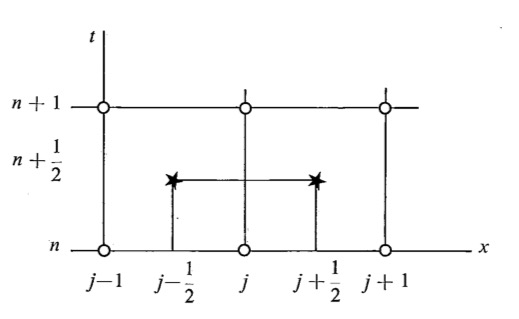
\includegraphics[width = .7 \textwidth]{figs/NM/pic11.jpg}
 \caption{} \label{fig:}
\end{figure}

provisional values are calculated at the centres of the two rectangular
meshes of this stencil, for points denoted by x signs. This is done
using centered space and forward time differencing, taking for
\(u_{j + \frac{1}{2}}^{n}\) and \(u_{j - \frac{1}{2}}^{n}\) arithmetic
averages of the values \(u_{j}^{n}\) at the two nearest grid points.
Therefore,

 \[\frac{u_{j + \frac{1}{2}}^{n + \frac{1}{2}} - \frac{1}{2}\left( u_{j + 1}^{n} + u_{j}^{n} \right)}
{\frac{1}{2}\Delta t} = - c \frac{u_{j + 1}^{n}{+ u}_{j}^{n}}{\Delta x}\]\[\frac{u_{j - \frac{1}{2}}^{n + \frac{1}{2}} - \frac{1}{2}\left( u_{j}^{n} + u_{j - 1}^{n} \right)}{\frac{1}{2}\Delta t} = - c \frac{u_{j}^{n}{- u}_{j - 1}^{n}}{\Delta t}\]

Using these provisional values another step is made, centered in both
space and time; thus

 \[\frac{u_{j}^{n + 1}{- u}_{j}^{n}}{\Delta t} =
- c \frac{u_{j + \frac{1}{2}}^{n + \frac{1}{2}} - u_{j - \frac{1}{2}}^{n + \frac{1}{2}}}{\Delta x}\]

Substitution of the provisional values from \texttt{a1.25} into this
equation gives

 \[\frac{u_{j}^{n + 1}{- u}_{j}^{n}}{\Delta t} =
- c\frac{u_{j + 1}^{n} + u_{j - 1}^{n}}{2\Delta x} +
\frac{1}{2}c^{2}\Delta t\frac{u_{j + 1}^{n} - 2u_{j}^{n} + u_{j - 1}^{n}}
{\left( 2\Delta x \right)^{2}}\]

It is interesting to note that this finite difference equation is very
similar to \texttt{a1.18}, that is, to the scheme obtained using simple
centered space differencing and the Matsuno time differencing. The only
difference is in the last term. This again approaches zero as
\(\Delta x,\Delta t \rightarrow 0\). However, if
\(\Delta x \rightarrow 0\) with \(\Delta t\) fixed, it now approaches
\(\frac{1}{2}c^{2}\Delta t\left( \frac{\partial^{2}u}{\partial x^{2}} \right)\).
Thus, we see that it is again equivalent in form to a finite difference
approximation to the Fickian diffusion term, but with a coefficient of
half the size given by \texttt{a1.18}. Furthermore, this term is now
calculated over an interval of \(2\Delta x\), and its damping effect
will be a maximum at that wave length. This sort of dependence on wave
length is often considered desirable for damping in a finite difference
scheme. This is because, as we will see later, there are serious
problems with finite difference calculations for small wave lengths,
especially around \(2\Delta x\). It is often possible to alleviate these
problems by using a dissipative scheme, which damps the
two-grid-interval waves preferentially.

While \texttt{a1.18} was of the first order of accuracy in time,
\texttt{a1.27} has truncation error

\(O\left\lbrack \left( \Delta x \right)^{2} \right\rbrack + O\left\lbrack \left( \Delta t \right)^{2} \right\rbrack\);

thus, it is of second order accuracy in both space and time.

To test the stability of the Lax-Wendroff scheme, we substitute

 \[u_{j}^{n} = Re\left\lbrack U^{\left( n \right)}e^{i  k  j \Delta x} \right\rbrack\]

Into \texttt{a1.27}. This gives

 \[U^{\left( n + 1 \right)} = \left\lbrack 1 + \mu^{2}\left( \cos{k\Delta x - 1} \right) -
i\mu\sin{k\Delta x} \right\rbrack U^{\left( n \right)}\]

Therefore

 \[\lambda = 1 + \mu^{2}\left( \cos{k\Delta x - 1} \right) - i\mu\sin{k\Delta x}\]

Since

\[\cos{k\Delta x - 1} = - 2\sin^{2}\frac{k\Delta x}{2}\]\[\sin{k\Delta x} = 2\sin\frac{k\Delta x}{2}\cos\frac{k\Delta x}{2}\]

we finally obtain

 \[|\lambda| = \left\lbrack  1 - 4\mu^{2}( 1 - \mu^{2} )\sin^{4}\frac{k\Delta x}{2} \right\rbrack^{1/2}\]

The expression within the bracket is a sum of two squares and never
negative. Thus, the Lax-Wendroff scheme is stable for
\(1 - \mu^{2} \geq 0\) or, for

\[\left| c \right|\frac{\Delta t}{\Delta x} \leq 1\]

This is again the Courant-Friedrichs-Lewy stability criterion
\texttt{a1.10}. The scheme is damping for

\[\left| c  \right|\frac{\Delta t}{\Delta x} < 1\]

It is instructive to analyze in some detail the dependence of the
damping wave length and on \(\mu\). For the shortest resolvable wave
length of \(2\Delta x\) we have \(k\delta x = \pi\) , and, therefore,

 \[|\lambda|  = \left( 1 - 4\mu^{2} + 4\mu^{4} \right)^{\frac{1}{2}} = \left| 1 - 2\mu^{2} \right|\]

For waves of twice the wave length,
\(4\Delta x,k\Delta x = \frac{\pi}{2}\),

and

 \[|\lambda| = \left( 1 - \mu^{2} + \mu^{4} \right)^{\frac{1}{2}}\]

In general, since

\[\frac{d|\lambda|}{\text{dμ}} = \frac{4\mu\left( 1 - 2\mu^{2} \right)\sin^{4}\frac{k\Delta x}{2}}{\left\lbrack 1 - 4\mu^{2}\left( 1 - \mu^{2} \right)\sin^{4}\frac{k\Delta x}{2} \right\rbrack^{\frac{1}{2}}}\]

all the \(|\lambda|\) curves have minima at \(\mu = 1/\sqrt{2}\).
Substituting this value of \(\mu\) into \texttt{a1.31} we find that
these minimum values of the amplification factor are equal to

 \[\left( 1 - \sin^{4}\frac{k\Delta x}{2} \right)^{\frac{1}{2}}\]

Thus, as the wave length increases from the minimum value of
\(2\Delta x\) this minimum value of \(|\lambda|\) monotonically
increases from zero and approaches unity as the wave length leads to
infinity.

The amplification factors for wave lengths of \(2\Delta x\) and
\(4\Delta x\) , as calculated in \texttt{a1.32} and \texttt{a1.33}, are
shown in \texttt{figg:12}. The amount of damping is seen to be
generally quite large for shorter wave lengths, especially for the wave
length \(2\Delta x\) . The amount of damping also depends on the time
step and the advection velocity. This is a disadvantage of the
Lax-Wendroff scheme because there is no reason why the amount of damping
should depend on these quantities and it is either impractical or
impossible to control the damping by changing them. For example, for
small values of \(\mu\) expansion of \texttt{a1.31} gives

\[|\lambda| = 1 - 2\mu^{2}\sin^{4}\frac{k\Delta x}{2} + \ldots\]

showing that for a given amount of time (a fixed value of
\(\n \Delta t\) the total damping will be approximately
proportional to \(\Delta t\). However, we wish to choose \(\Delta t\)
to give the best accuracy and stability properties, not to give the
optimal amount of damping.

\begin{figure}
 \centering
 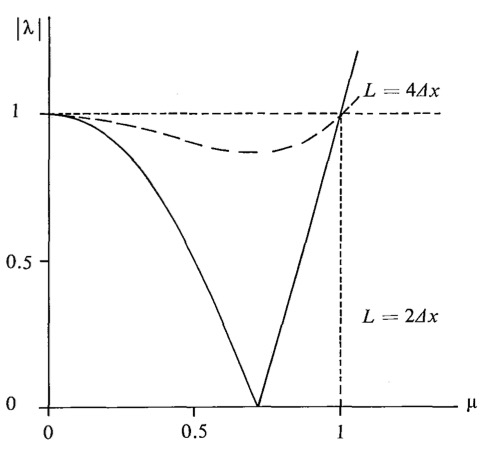
\includegraphics[width = .7 \textwidth]{figs/NM/pic12.jpg}
 \caption{} \label{fig:}
\end{figure}

The Lax-Wendroff scheme has been fairly widely used in atmospheric
models, due to a recommendation by Richtmyer (1963), and its reasonably
good behaviour. It is second order accurate, explicit, not
unconditionally unstable, and since it is a two levels scheme there is
no computational mode. None of the schemes obtained by combining
centered space differencing with one of the seven time differencing
schemes studied in chapter \texttt{Chapter2} has all of these
advantages. The dissipation of the Lax-Wendroff scheme will not be
harmful if its total effect is negligible compared with the physical
dissipation, and it can also be useful for controlling the shortest
waves. If the physical dissipation is very small or non-existent, it is
better to use a neutral scheme.

One should point out here that we can change the time differencing
scheme intermittedly during an integration, so as to get the required
amount of a particular effect. For example, in the general circulation
model developed at the National Center for Atmospheric Research,
Boulder, Colo., the Lax-Wendroff scheme is used because of its damping
effect on the shortest waves. However, to keep the amount of damping
small, it is used only once in every hundred steps, the rest are made
using a neutral leapfrog scheme (Kasahara, 1969). On the other hand, in
the British operational model (e.g. Gadd, 1974b) the Lax-Wendroff scheme
is used every time step, with the authors of the model making no mention
of any excessive damping due to the scheme for the purposes of that
model

\section{Computational dispersion}\label{sec:computational-dispersion}

As we have seen, the linear advection equation

 \[\frac{\partial u}{\partial t} + c\frac{\partial u}{\partial x} = 0\]\[c = const\]

has a solution in the form of a single harmonic component

 \[u\left( x,t \right) = Re\left\lbrack U\left( t \right)e^{\text{ikx}} \right\rbrack\]

provided that

 \[\frac{\text{dU}}{\text{dt}} + ikcU = 0\]

In this oscillation equation \(kc\) is equal to the frequency \(\nu\),
and \(c = \frac{\nu}{k}\) is the phase speed of the waves. It is seen
that waves of all wave lengths are propagated with the same phase speed,
that is, the function \(u\left( x,t \right)\) is advected with no change
in shape at a constant velocity \emph{c} along the \emph{x} axis. There
is no dispersion.

Now consider the equation

 \[\frac{{\partial u}_{j}}{\partial t} + c\frac{u_{j + 1} - u_{j - 1}}{2\Delta x} = 0\]

that is obtained by approximating the space derivative in \texttt{a2.1}
by a centered difference quotient. The equation \texttt{a2.4} is neither
a differential nor a difference equation, but a hybrid of these two. An
equation of this type can be called a differential-difference equation,
or a semi discrete equation. The finite difference equations obtained
when the time derivative in \texttt{a2.4} is approximated using a
consistent time differencing scheme will approach (\texttt{a2.4} as the
time step approaches zero. Thus, for small \(\Delta t\) \texttt{a2.4}
represents an approximation to these finite difference equations. Since
the time derivative has retained its differential form, any error in
\texttt{a2.4} is due to the space differencing.

For this reason, equations of this type are used to study the effect of
particular space difference approximations on the properties of the
numerical solution.

Recall that \texttt{a2.4} has a solution in the form of a single
harmonic component

 \[u_{j}\left( t \right) = Re\left\lbrack U\left( t \right)e^{\text{ikjx}} \right\rbrack\]

provided that

 \[\frac{\text{dU}}{\text{dt}} + ik\left( \frac{\sin{k\Delta x}}{k\Delta x} \right)U = 0\]

We have now written this so that it can conveniently be compared with
\texttt{a2.3} . Instead of the constant phase speed c, we see that waves
now propagate with the phase speed

 \[c^{*} = c\frac{\sin{k\Delta x}}{k\Delta x}\]

This phase speed is a function of the wave number k. Thus, the finite
differencing in space causes a dispersion of the waves ; we shall call
this effect \emph{computational dispersion}. As \(k\Delta x\) increases
from zero, the phase speed \(c^{*}\) monotonically decreases from c, and
becomes zero for the shortest resolvable wave length \(2\Delta x\), when
\(k\Delta x = \pi\). Thus, all waves propagate at a speed that is less
than the true phase speed c, with this decelerating effect increasing as
the wave length decreases. The two-grid-interval wave is stationary.

The reason for the two-grid-interval wave being stationary is obvious
when we look at the plot of that wave, shown in \texttt{figg:13}. For
this wave \(u_{j + 1} = u_{j - 1}\) at all grid points, and
\texttt{a2.4} gives a zero value for
\(\frac{{\partial u}_{j}}{\partial t}\)

We have encountered two effects here. Firstly, the advection speed is
less than the true advection speed. The consequence of this error is a
general retardation of the advection process. Secondly, the advection
speed changes with wave number; this false dispersion is particularly
serious for the shortest waves.

\begin{figure}
 \centering
 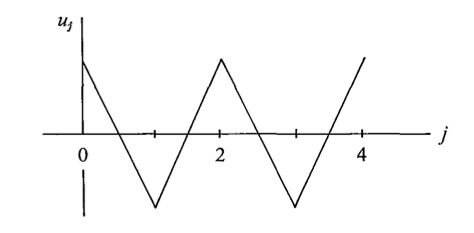
\includegraphics[width = .7 \textwidth]{figs/NM/pic13.jpg}
 \caption{} \label{fig:}
\end{figure}

If the pattern that is being advected represents a superposition of
more than one wave, this false dispersion will result in a deformation
of that pattern. It is especially small-scale patterns in the
atmosphere, e.g. fronts, shear lines, etc., that represent a
superposition of many waves, including a significant proportion of the
shortest waves. For this reason, in numerical forecasting, such
patterns, if present in the initial fields, are fairly rapidly deformed,
until they aquire a form which is less sharp than in the beginning.
Since such small-scale features are of particular importance in weather
processes, the effect of computational dispersion deserves very careful
consideration.

We now turn our attention to the group velocity. In the case of the
linear equation \texttt{a2.1} we obtain for the group velocity \(c_{g}\)

 \[\tau_{c} = \frac{d\left( \text{kc} \right)}{\text{dk}} = c\]

Thus, the group velocity is constant and equal to the phase speed \(c\).
With the differential-difference equation \texttt{a2.4} , however,
\texttt{a2.7} gives for the group velocity c*

 \[c_{g} = \frac{d\left( kc^{*} \right)}{\text{dt}} = c\cos{k\Delta x}\]

Thus, as \(k\Delta x\), increases from zero, the group velocity
\(c_{g}\), decreases monotonically from \(c_{g}\), and becomes equal
\({- c}_{g}\) for the shortest resolvable wave length of
\(2k\Delta\text{x.}\)

These results are summarized in \texttt{figg:14}. For the exact
advection equation \texttt{a2.1} both individual waves and wave packets,
that is, places where superposition of waves results in a maximum
amplitude of a group of neighbouring wave numbers, propagate at the same
constant velocity \(c = c_{g}\). Introduction of the centered space
finite difference quotient in (2.4) both makes the phase speed and the
group velocity decrease as the wave number increases. The error is
particularly great for the shortest resolvable wave lengths; waves with
wave lengths less

\begin{figure}
 \centering
 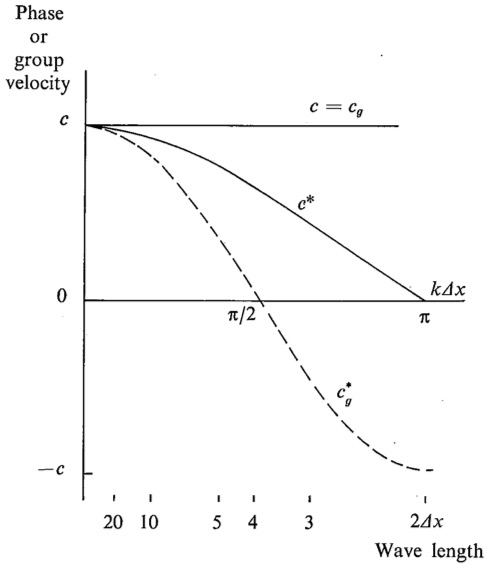
\includegraphics[width = .7 \textwidth]{figs/NM/pic14.jpg}
 \caption{} \label{fig:}
\end{figure}

Than \(4\Delta x\) even have a negative group velocity. This means that
wave packets made up of these waves propagate in the direction opposite
to the advection velocity and opposite to the direction of propagation
of individual waves.

This situation can be illustrated by a simple example. Let us define Y
(x) as a function that is slowly varying in space; for example, it can
be a sine function of a large wavelength. Furthermore, we define

 \[u_{j} \equiv \left( - 1 \right)^{j}Y_{J}\]

as shown in \texttt{figg:15}. Thus, the function ±Y(x) is the envelope
of the function \(u_{j}\). Suppose that we calculate the advection of
\(u_{j}\) using \texttt{a2.4} , then substituting \texttt{a2.10} into
\texttt{a2.4} we obtain

\[\frac{\partial Y}{\partial t} - c\frac{Y_{J + 1} - Y_{J - 1}}{2\Delta X} = 0\]

Thus, the advection of \(Y_{j}`is governed by the same equation
as the advection of :math:`u_{j}`except that the advection velocity
appears with an opposite sign ! Therefore, as the individual short waves
of the function :math:`u_{j}\) slowly propagate in the direction of the
positive x axis, the envelope \(\pm Y\left( x \right)\), which has a
long wave length, propagates relatively fast in the opposite direction.
When it is a sine function, so that it consists of a single harmonic, it
propagates with no change in shape. Because of (2.10), u\} must also be
advected with no change in shape ; from this we conclude that u\} also
consists of a single harmonic component. If, on the other hand, the
function \(Y\left( x \right)\) consisted of a number of harmonic
components, the shapes of both \(Y( x )\) and \(u_{j}\) would change
during the advection process, as a result of the computational
dispersion of these components.

It is possible to obtain an analytic solution of \texttt{a2.4} , which
can be used to analyze its behaviour for some given initial conditions
of interest. To this end it is convenient to define a non-dimensional
time variable

 \[\tau \equiv \frac{\text{ct}}{\Delta x}\]

\begin{figure}
 \centering
 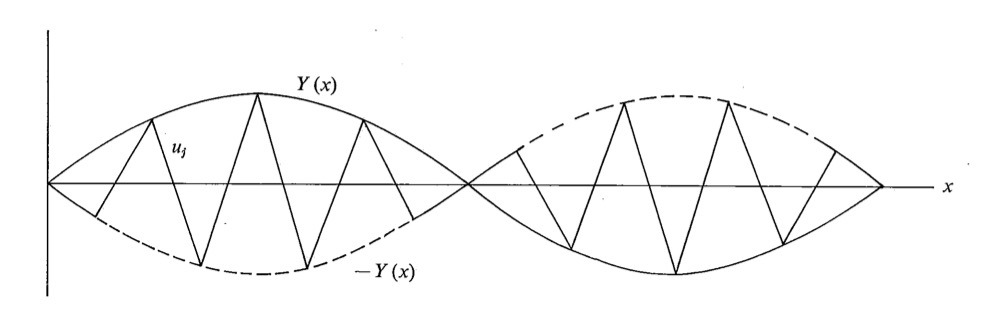
\includegraphics[width = .7 \textwidth]{figs/NM/pic15.jpg}
 \caption{} \label{fig:}
\end{figure}

and, after dividing equation \texttt{a2.4} by \(\frac{c}{2\Delta x}\),
to write it in the form

 \[2\frac{d}{d\tau}u_{j}\left( \tau \right) = u_{j - 1}\left( \tau \right) - u_{j + 1}\left( \tau \right)\]

This can be recognized as the recurrence formula of the Bessel function
of the first kind of order \(j,J_{j}\left( \tau \right)_{,}\) (e.g.
Courant and Hilbert, 1953, p. 488). In other words,

 \[u_{j}\left( \tau \right) = J_j\left( \tau \right)\]

is a solution of \texttt{a2.12}. Several of these functions, of the
lowest order, are shown in \texttt{figg:16}. The figure illustrates more
of these functions than indicated, since, for any \(j\),

\[J_{- j} = \left( - 1 \right)^{j}J_{j}\]

Note, furthermore, that in \texttt{a2.12} the subscript \emph{j} can
take any integer value, since the location of the grid point for which
we choose \(J = 0\) is arbitrary. Thus, a solution that is more general
than \texttt{a2.13} is

\[u_{j}\left( \tau \right) = J_{j - p}\left( \tau \right)\]

\begin{figure}
 \centering
 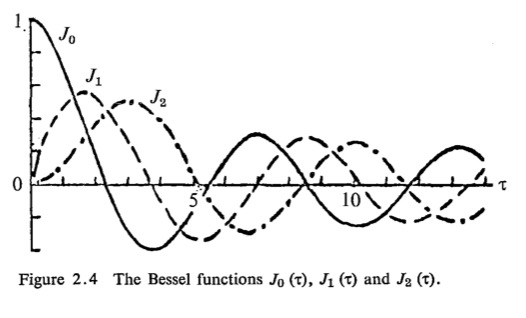
\includegraphics[width = .7 \textwidth]{figs/NM/pic16.jpg}
 \caption{} \label{fig:}
\end{figure}

Where \(p\) is an arbitrary integer. Since we are solving a linear
equation, a still more general solution is a linear combination of all
these solutions, that is

 \[u_{j}\left( \tau \right) = \sum_{p = - \infty}^{\infty}{a_{p}J_{j - p}}\left( \tau \right)\]

where \(a_{p}\) are arbitrary constants. Now, for \(\tau = 0\) all of
the functions \(J_{k}\) are equal to zero, except \(J_{0}\), for which
\(J_{0}\left( 0 \right) = 1\). Hence, substituting \(\tau = 0\) into
\texttt{a2.14} we obtain

 \[u_{j}\left( 0 \right) = a_{j}\]

Therefore the constants in \texttt{a2.14} can be chosen so as to satisfy
arbitrary initial conditions \(u_{j} = u_{j}\left( 0 \right)\). Since it
can satisfy arbitrary initial conditions, \texttt{a2.14} is seen to
represent the general solution of \texttt{a2.12}, or \texttt{a2.4}.

It is instructive to look in some detail at the solution satisfying the
initial conditions

 \[\begin{aligned}
     u_{j}\left( 0 \right) = \left\{ \begin{array}{cc}
                                      1  &  for \quad j = 0\\
                                      0  &  for \quad j \neq 0\\
     \end{array} \right.
\end{aligned}\]

the simplest solution of the form \texttt{a2.13}, for different values
of the non-dimensional time. At the initial moment the function u\}
consists of a single pulse-like disturbance, centered at the point
\(j = 0\), as shown in the upper diagram of \texttt{figg:17}. We note
that, because of \texttt{a2.12}, \(\frac{\text{du}_{j}}{\text{dt}}\) is
then equal to zero at all points except at \(j = - 1\) and \(j = 1\),
where it is equal to 1/2 and 1/2, respectively.

Thus, at the initial moment the disturbance propagates at the same rate
in the directions of both the positive and the negative x axis. Further
propagation of the disturbance according to \texttt{a2.13} can be
followed using \texttt{figg:8}, or, more accurately, using some tables
of Bessel functions. Solutions obtained in this way for \(\tau = 5\) and
\(\tau = 10\) are shown in the middle and lower diagrams of
\texttt{figg:17}, respectively.

\begin{figure}
 \centering
 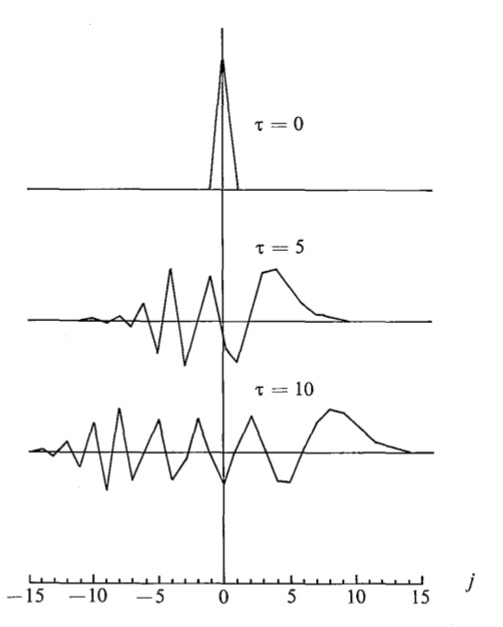
\includegraphics[width = .7 \textwidth]{figs/NM/pic17.jpg}
 \caption{} \label{fig:}
\end{figure}

The three diagrams present an example of the computational dispersion
of the second-order centered space differencing. We note that if we
expand a single pulselike disturbance as a cosine Fourier integral

\(u\left( x \right) = \int_{0}^{\infty}{a\left( k \right)\cos\text{kxdk}}\),

\(a\left( k \right) = \frac{2}{\pi}u\left( x \right)\cos\text{kxdx}\),

and a(k) is calculated numerically using the grid point values only, we
obtain a constant value

\(a\left( k \right) = \frac{2}{\pi}\Delta x\)

Therefore, all the harmonic components have equal amplitude. By analogy
with the light spectrum, such a function is called white noise if it
does not appear for physical reasons. Its Fourier components are
advected with different phase speeds, as summarized in \texttt{figg:14},
bringing about a dispersion of the disturbance. With the non-dimensional
time chosen here we see from \texttt{a2.12} that the physical advection
velocity should keep the pulse located at the point \(j = \tau.\)
Because of the space difference approximation, however, all the phase
speeds are less than the physical advection velocity. The main
disturbance, as seen in \texttt{figg:17}, is advected at a speed only
slightly less than the physical one ; obviously it mostly consists of
the longer wave components, which have an advection speed not much
different from the physical advection velocity. However, it is seen to
be diffusing away with time, which is again a result of the dispersion.
We also observe propagation of a group of short waves in the direction
opposite to that of the physical advection. Since the appearance of
these waves contradicts the physical properties of the advection
equation, such waves are called parasitic waves.

The solution of the differential-difference equation is, obviously,
quite unsatisfactory as an approximation to the true solution. However,
this example, with the initial disturbance located at one point only, is
completely unsuitable for a good solution by a difference
approximation. This is exactly the reason why it provides an
instructive illustration of the difficulties involved.

Analytic solutions for a more general case, when a centered difference
approximation is made to the time derivative also have been considered
by Egger (1971).

\section{Schemes with uncentered space differencing}\label{sec:schemes-with-uncentered-space-differencing}

The space derivative in \texttt{a2.1} can also be approximated using
uncentered differencing. Still using values at two points for this
approximation it is attractive for physical reasons to have one of these
points as the central point and the second located on the side from
which the fluid is being advected toward the centre. Therefore we
approximate \texttt{a2.1} by

 \[\begin{aligned}
     \frac{\partial u_j}{\partial t} + c\frac{u_{j} - u_{j - 1}}{\Delta x} &= 0, \quad \textrm{for}
     \quad c > 0 \\
\end{aligned}\]\[\begin{aligned}
                  \frac{\partial u_j}{\partial t} + c\frac{u_{j+1} - u_{j}}{\Delta x} &= 0 \quad \textrm{for}
                  \quad c < 0 \\
\end{aligned}\]

These equations are again differential-difference equations. The first
equation in \texttt{a3.1} employs the backward and the second in
\texttt{a3.1} the forward difference quotient for the approximation to
the space derivative. However, in both cases the differences are
calculated on the side from which the advection velocity reaches the
centre; hence, these differences are called \emph{upstream differences}.
Calculated on the opposite side the differences would be called
downstream differences.

Eqs. \texttt{a3.1} can be used to construct schemes for the advection
equation, by approximating the time derivative by one of the many
possible consistent methods. The resulting schemes will only be of the
first order of accuracy. However, they have a particular advantage over
centered schemes in space when applied to the advection of a disturbance
similar to the one considered in the preceding section. This is that,
with upstream differences, a disturbance cannot propagate in the
direction opposite to the physical advection. Thus, no parasitic waves
will contaminate the numerical solution.

If, specifically, a forward difference is used for the time derivative
in \texttt{a3.1}, we obtain, for \emph{c \textgreater{} 0},

 \[\frac{u_j^{n + 1} - u_j^{n}}{\Delta t}
+c \frac{u_j^{n} - u_{j - 1}^{n}}{\Delta x} = 0\]

This is the scheme that was used for the examples of the introductory
chapter. It was found that this scheme was damping, with the amount of
damping depending on the wave length, with a maximum for the shortest
resolvable wave length of \(2\Delta x\). The analytic solution of the
difference equation \texttt{a3.2} has been discussed by Wurtele (1961).

The advantage that is accomplished, at least in principle, by using
upstream differencing as compared with centered or downstream
differencing, can be illustrated by considering the \emph{domain of
influence} of a grid point in different schemes. We still consider the
case \emph{c \textgreater{} 0}.

\begin{figure}
 \centering
 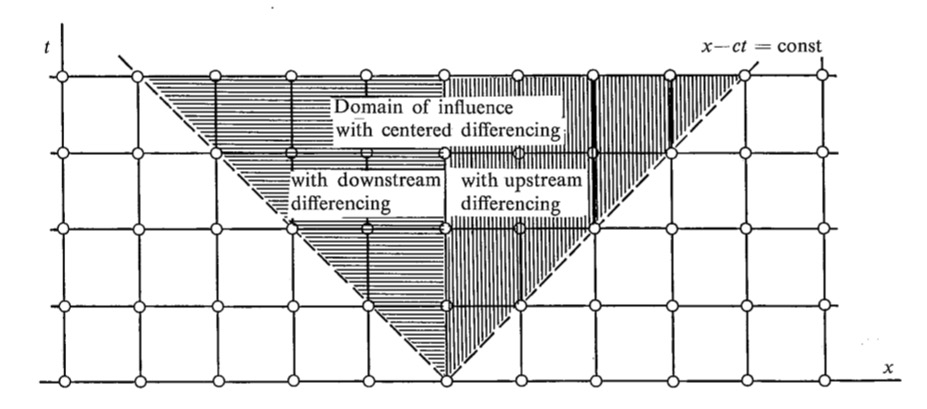
\includegraphics[width = .7 \textwidth]{figs/NM/pic31.jpg}
 \caption{} \label{fig:}
\end{figure}

In the true solution, a grid point value can be said to propagate along
the characteristic \emph{x - ct} = const. \texttt{figg:31} shows a grid
point marked by a circle with the associated characteristic passing
through it. With upstream differencing as in \texttt{a3.2}, the value at
that grid point will influence the values at points within the domain
shaded by vertical lines. The figure also shows the domains of influence
with centered and downstream differencing. Of the three domains of
influence, that given by upstream differencing is clearly the best
approximation to the characteristic line representing the domain of
influence in the true solution.

This discussion suggests constructing a scheme for \texttt{a2.1} by
tracing a characteristic back from the point
\(\left( j\Delta x,\left( n + 1 \right)\Delta t \right)\) to intersect
the previous time level \(\tau = n\Delta t\) and calculating the value
\(u^{*}\) at the point of intersection by interpolation. We then set
\({u_{j}^{n + 1} = u}^{*}\). Choosing a linear interpolation procedure,
that employs values at two neighbouring points at the time
\(n\Delta t\), we obtain

\(u_{j}^{n + 1} = u_{j - 1}^{n} + \frac{u_{j}^{n} - u_{j - 1}^{n}}{\Delta x}\left( \Delta x - c\Delta t \right)\)

This can be identical to the scheme \texttt{a3.2}, with upstream
differencing. If, on the other hand, a quadratic interpolation procedure
is chosen, using three neighboring points, one obtains the Lax-Wendroff
scheme, as the reader can readily verify.

For further insight into the properties of schemes that can be obtained
from \texttt{a3.1} we consider the analytic solution of this
differential-difference equation. For small values of \(\Delta t\) this
will approximate the solution obtained from the difference schemes. As
before we introduce the non-dimensional time
\(\tau = \frac{\text{ct}}{\Delta x}\). Eq. \texttt{a3.1} can then be
written as

 \[\frac{d}{d t}u_{j}\left( \tau \right) + u_{j}\left( \tau \right) - u_{j - 1}\left( \tau \right) = 0\]

A solution of this equation is the Poisson frequency function

 \[
  \begin{aligned}
     u_j(\tau) = \left\{ \begin{array}{cc}
                          \frac{e^{- \tau}\tau^{j - p}}{(j-p)!} \qquad &\textrm{for} \quad j \geq p \\
                           0  \qquad &\textrm{for} \quad j < p \\
     \end{array} \right.
\end{aligned}
 \]

as can easily be checked by substitution. Here \emph{p} is again an
arbitrary integer, that is, we have already taken into account the fact
that the location of the point \emph{j} = 0 is arbitrary.

\begin{figure}
 \centering
 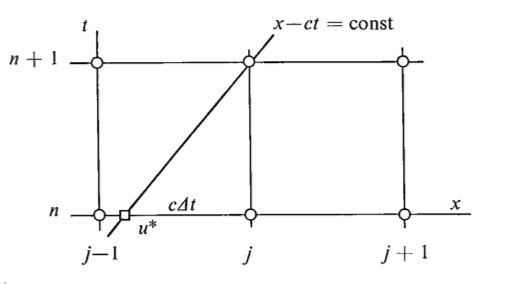
\includegraphics[width = .7 \textwidth]{figs/NM/pic32.jpg}
 \caption{} \label{fig:}
\end{figure}

\begin{figure}
 \centering
 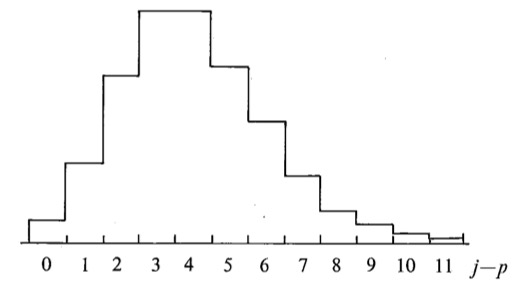
\includegraphics[width = .7 \textwidth]{figs/NM/pic33.jpg}
 \caption{The Poisson frequency function \texttt{a3.4}, for the case
  \(\tau = 4\).}
\end{figure}

An example of the Poisson frequency function is shown in
\texttt{figg:33}; the graph in the figure represents the shape of this
function for \(\tau = 4\). There is no need to include a vertical scale,
since the area enclosed by the graph of a frequency function has to be
equal to unity, so

 \[\sum_{j - p = 0}^{\infty}\frac{e^{- \tau}\tau^{j - p}}{\left( j - p \right)^{!}} = 1\]

Thus, for \(\tau = 0\), when, as shown by \texttt{a3.4}, the histogram
consists of a single rectangle, its ordinate is equal to unity.

Consider now the change in shape of the histogram \texttt{a3.4} as the
non-dimensional time \(\tau\) increases from zero. The initial shape of
this histogram, that of a parallelogram having a base \(\Delta x\) and
erected at a single grid point, is, of course, equivalent to the shape
of the pulse-like disturbance \texttt{a2.16} used for the example of the
previous section. As I increases beyond zero \texttt{a3.4} transforms
into a skewed bell-shaped histogram of the type as shown in the figure,
with its mean position on the \emph{x} axis

\[\sum_{j - p = 0}^{\infty}\left( j - p \right)\frac{e^{- \tau}\tau^{j - p}}{\left( j - p \right)^{!}} = \tau\]

moving at a constant speed. Thus, the mean position propagates with a
speed equal to the physical advection velocity. The maximum point of the
histogram, however, lags behind as is shown by the skewed shape of the
histogram. Physically unjustified negative values of \(u_{j}\), never
occur and no parasitic waves appear on the opposite side of zero from
the direction of the physical advection. Furthermore, as follows from
\texttt{a3.5}, the total amount of the advected quantity is exactly
conserved. However, the disturbance is damped out during the advection
process at quite a high rate.

As in Section \texttt{Section3.2} we can form a solution more general
than \texttt{a3.4}, as a linear combination of all possible solutions
\texttt{a3.4}, that is

 \[u_{j}\left( \tau \right) = \sum_{p = - \infty}^{j}a_{p}\frac{e^{- \tau}\tau^{j - p}}{\left( j - p \right)^{!}}\]

where \(a_{p}\) are arbitrary constants. Substituting \(\tau = 0\) into
\texttt{a3.6} we obtain

 \[u_{j}\left( 0 \right) = a_{j}\]

Thus, the constants \(a_{p}\) can again be chosen so as to satisfy
arbitrary initial conditions \(u_{j} = u_{j}(0)\), and so \texttt{a3.6}
represents the general solution of \texttt{a3.3}, or \texttt{a3.1}.
Considering the behaviour of the simple solution \texttt{a3.4}, and the
summation limits in \texttt{a3.6}, we see that in general the value
\(u_{j}\left( \tau \right)\) at a point \emph{j} can be considered as a
result of superposition of the effect of the initial values at that
point and of the initial values at all the points located
\emph{upstream} of it.

An example of the solutions \texttt{a2.14}, for centered differencing,
and \texttt{a3.6}, for upstream differencing, for an initial disturbance
of a somewhat larger space scale

\[\begin{aligned}
   u_{j}(0) = \left\{ \begin{array}{cc}
                       1  &\textrm{for} \quad j = -1,0,1\\
                       0  &\textrm{for} \quad j \neq -1,0,1\\
   \end{array} \right.
\end{aligned}\]

is shown in \texttt{figg:34}. If the grid distance is of the order of
300 km, and c is about 15 msec-1 we can see that 5 units of
non-dimensional time approximately correspond to the physical time of
one day. Thus, the damping effect of the upstream differencing is seen
to be quite severe. The figure also illustrates the properties of the
two methods described, but to a lesser extent than the examples with the
initial disturbance limited to a single grid point only. Thus we can
hardly claim that the use of upstream differencing instead of centered
second-order differencing has, generally speaking, improved the
solution.

\begin{figure}
 \centering
 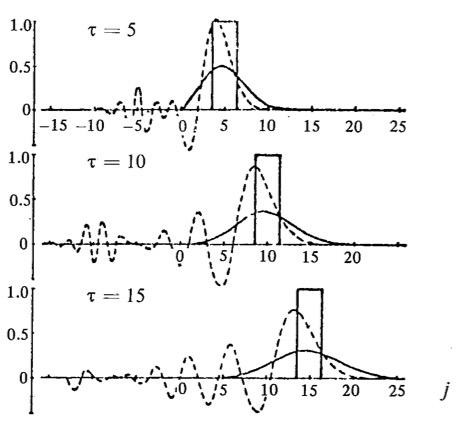
\includegraphics[width = .7 \textwidth]{figs/NM/pic34.jpg}
 \caption{} \label{fig:}
\end{figure}

\section{Schemes with centered fourth-order
space
differencing}\label{sec:schemes-with-centered-fourth-order-space-differencing}

Most of the difficulties that have been discussed in this chapter, in
particular the phase speed error and the computational dispersion, have
been due to the approximations used for space differencing. Thus,
consideration should be given to other possibilities; one is to employ
approximations of a higher order of accuracy. We shall first construct
such an approximation.

When the approximate value \(u_{j}\) are expanded into Taylor series
about the central point, and substituted into the finite difference
quotient, we obtain

 \[\frac{u_{j + 1} - u_{j - 1}}{2\Delta x} = \frac{\partial u}{\partial x} +
\frac{1}{3!}\frac{\partial^3 u}{\partial x^3}( \Delta x )^{2} +
O\left\lbrack \left( \Delta x \right)^{4} \right\rbrack \]

Thus, this quotient is of the second order of accuracy. It is formed by
taking differences of values of \(u_{j}\) at points one grid distance
away from the central point. Similarly a quotient can be formed by
taking differences of values two grid distance away. We then obtain,
replacing \(\Delta x\) in \texttt{a4.1} by \(2\Delta x\),

\[\frac{u_{j + 2} - u_{j - 2}}{4\Delta x} = \frac{\partial u}{\partial x} +
\frac{4}{3!}\frac{\partial^3 u}{\partial x^3}( \Delta x )^{2} +
O\left\lbrack \left( \Delta x \right)^{4} \right\rbrack\]

This quotient is still second order accurate, but the coefficients are
larger. Other consistent approximations to
\(\frac{\partial u}{\partial x}`can be formed as linear
combinations of the quotients :eq:`a4.1\) and \texttt{a4.2}. The
combination for the second order terms in the truncation errors of
\texttt{a4.1} and \texttt{a4.2} cancel is particularly important. This
is

\[\frac{4}{3}\frac{u_{j+1} - u_{j-1}}{2\Delta x} - \frac{1}{3}\frac{u_{j+2} - u_{j-2}}{4\Delta x}
= \frac{\partial u}{\partial x}
+ O\left\lbrack \left( \Delta x \right)^{4} \right\rbrack\]

And represets a fourth-order accurate approximation to
\(\frac{\partial u}{\partial x}\).

We can also think of the approximation \texttt{a4.3} as representing a
linear extrapolation of the quotients \texttt{a4.2} and \texttt{a4.1} so
as to simulate an approximation corresponding to differences taken
between points at a distance \emph{d} less than \(\Delta x\) away from
the centre. A simple calculation shows that the approximation
\texttt{a4.3} is obtained by extrapolation for the value
\(d = \frac{2\Delta x}{3}\). Of course, there is no reason to expect
that the accuracy of such an approximation should decrease monotonically
as \emph{d} decreases.

We now want to look at the effect on the phase speed of using the
approximation \texttt{a4.3} for the space derivative in the advection
equation. Replacing the space derivative in \texttt{a2.1} by
\texttt{a4.3} we obtain the differential-difference equation

\[\frac{\partial u_{j}}{\partial t} + c\left( \frac{4}{3}\frac{u_{j + 1} - u_{j - 1}}{2\Delta x} - \frac{1}{3}\frac{u_{j + 2} - u_{j - 1}}{4\Delta x} \right) = 0\]

As in Section \texttt{Section3.2}, we investigate the behavior of a
tentative solution in form of a harmonic component

\[u_j( t ) = Re\left\lbrack U\left( t \right)e^{ikj\Delta x} \right\rbrack\]

With second-order space differencing, we obtain the phase speed

\[c^{*} = c\frac{\sin{k \Delta x}}{k \Delta x}\]

Now, in the same way, with fourth-order differencing we find the phase
speed

\[c^{**} = c\left( \frac{4}{3}\frac{\sin{k\Delta x}}{k \Delta x}
- \frac{1}{3}\frac{\sin{2k\Delta x}}{2k\Delta x} \right)\]

We shall compare these two results. For second order differencing, we
obtain by series expansion for small values of k

\[c^{*} = c\left( 1 - \frac{1}{3!}\left( k\Delta x \right)^{2} + \ldots \right)\]

On the other hand, with fourth order differencing we have

\[c^{**} = c\left( 1 - \frac{4}{5!}\left( k\Delta x \right)^{4} + \ldots \right)\]

Thus, even though the decelerating effect is still present, the phase
speed error has been much reduced for small values of \emph{k}.

These phase speeds are shown in \texttt{figg:41} as functions of
\(k\Delta x\), for all admissible values of \emph{k}. The figure
illustrates the very significant increase in accuracy of the phase
speed for large-scale and medium-scale waves. However, as the wave
length approaches its minimum value of \(2\Delta x\) the increase in
phase speed obtained by fourth order differencing diminishes, until,
finally, the wave with wave length \(2\Delta x\) is again stationary.

\begin{figure}
\centering
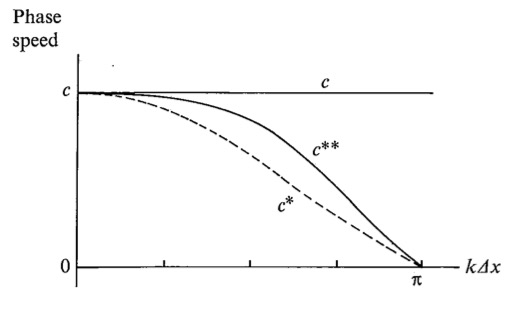
\includegraphics[width = .7 \textwidth]{figs/NM/pic41.jpg}
\caption{} \label{fig:}
\end{figure}

Moreover, for short waves the slope of the phase speed curve is greater
than with second order differencing, and, therefore, the computational
dispersion of these waves is greater. Thus, although a short wave-length
disturbance will now be advected at a somewhat greater speed its false
deformation, due to computational dispersion, will be faster.

Because of the decrease in the phase speed error of the longer waves,
the use of fourth order schemes for advection has brought about
significant improvements in operational numerical forecasting in both
the U.S.A. and Japan, in barotropic and quasi-geostrophic baroclinic
models. With primitive equation models, now in use in all advanced
forecasting centres, fourth order advection schemes are not yet quite so
widespread. Still, it is generally believed that fourth-order advection
schemes should be used in operational forecasting. However, the use of
advection schemes of a high-order of accuracy in general circulation
models may not be so important. The choice is between increasing the
accuracy of space differencing or spending an equivalent amount of extra
computation time in reducing the grid size of the model. A
straightforward calculation (e.g. Thompson, 1961, p. 157) shows that
the first alternative should be advantageous.

The use of the additional grid points needed for higher order
differencing does create some side difficulties. In much the same way as
using more than two levels for time differencing resulted in the
appearance of computational modes in time, so the use of additional
grid points for space differencing results in the appearance of
computational modes in space. Furthermore, formulation of boundary
conditions becomes more complicated. Simply formulated boundary
conditions may be a source of serious problems.

For small scale disturbances, of a scale close to two grid intervals in
space, no finite difference method is really satisfactory. Additional
ways of constructing difference schemes for the advection equation are
discussed in the paper by Anderson and Fattahi (1974) where further
references are given. If it is felt that, in a particular situation, the
improvement of the advection of scales close to two grid intervals is
necessary, the obvious method is to find a way of making the computation
with a reduced grid size. As can be inferred from \texttt{figg:41},
halving the grid size with simple second-order differencing makes the
stationary two-grid-interval wave move at a speed of almost 2/3 of its
physical advection speed. But this, of course, is not easily attainable:
in two-dimensional problems, halving the grid size increases the
computational time requirements by a factor of four, and, with the usual
time difference schemes by an additional factor of two in order to
maintain computational stability. Still, a steady increase in the
capabilities of commercially available computers enables constant
improvements of this kind, so that it is expected that in a few years
the resolution of atmospheric models may be such that advection errors
will not be a major problem. At present it is estimated that the
horizontal truncation errors in the advection terms are the largest
single source of errors in short range numerical forecasting, accounting
for almost 40 per cent of the total error (Robert, 1974).

Another way of improving the advection of small scale systems may be to
develop a computational method more in spirit of the Lagrangian system
of equations. As yet, such methods have not been very much explored in
meteorology.

\section{The two-dimensional advection equation}\label{sec:the-two-dimensional-advection-equation}

We now consider the two-dimensional linear advection equation

\[\frac{\partial u}{\partial t} + c_{x}\frac{\partial u}{\partial x}+ c_y\frac{\partial u}{\partial y} = 0
\qquad c_x,\quad c_y = cost\]

where \(u = u\left( x,y,t \right)`is a function of two space
variables, and :math:`c_{x},c_{y}\) are the components of the advection
velocity. Thus, the advection speed is given by

\[c = \sqrt{c_{x}^{2} + c_{y}^{2}}\]

We shall test the stability of schemes for the numerical solution of
\texttt{a5.1} by the procedure of Section \texttt{Section3.1}. Thus,
space derivatives are approximated by standard second-order difference
quotients, giving

\[\frac{\partial}{\partial t}u_{i,j} = - c_{x}\frac{u_{i + 1,j} - u_{i - 1,j}}{2\Delta x} - c_{y}\frac{u_{i,j + 1} - u_{i,j - 1}}{2\Delta y}\]

Here, as is usual for two-dimensional problems, we have changed the
choice of subscript denoting the grid points along \emph{x} axis, so
that the coordinates of the grid points are now \(x = i\Delta x\),
\(y = i\Delta y\), and approximate values
\(u\left( i\Delta x,j\Delta y \right)\) are denoted by \(u_{i,j}\). As a
tentative solution of \texttt{a5.3} we substitute

\[u_{i,j} = Re\left\lbrack U\left( t \right)e^{i ( kx + ly )} \right\rbrack
\]

giving the oscillation equation

\[\frac{d U}{d t} = i\left( - \frac{c_{x}}{\Delta x}\sin{k\Delta x} -\frac{c_{y}}{\Delta y}\sin{l\Delta y} \right)U\]

If the leapfrog scheme is used for the time derivative, we obtain as the
stability criterion

\[\left| \left( \frac{c_x}{\Delta x}\sin{k\Delta x} +
\frac{c_y}{\Delta y}\sin{l\Delta y} \right)\Delta t \right| \leq 1\]

This has to be satisfied for all admissible values of the wave numbers
\emph{k}, \emph{l}.

For simplicity, we shall consider only the cases where
\(\Delta x = \Delta y\) we denote this grid size by \(d^{*}\). In the
wave number plane, that is, a diagram with co-ordinates \emph{k, l}, the
admissible wave numbers are contained within the square region shown in
\texttt{figg:51}. Inside that region the maximum value of the left-hand
side of \texttt{a5.6} is obtained at the centre of the square, marked by
a circle. The wave represented by that point has wave lengths \(4d^*\)
in both the \emph{x} and \emph{y} directions so that
\(sink{\Delta x} = \sin{l\Delta y} = 1\).

\begin{figure}
\centering
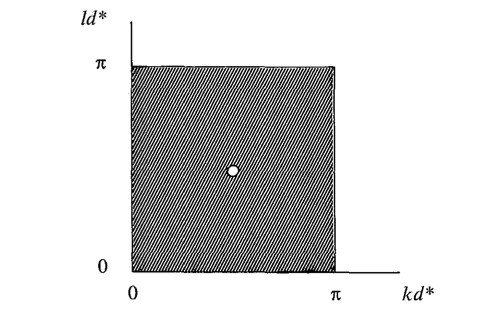
\includegraphics[width = .7 \textwidth]{figs/NM/pic51.jpg}
\caption{} \label{fig:}
\end{figure}

For a given value of the advection speed the left-hand side of
\texttt{a5.6} has a maximum value at this point if the advection
velocity makes an angle of \(\frac{\pi}{4}\) with the axis, in this case
\(c_{x} = c_{y} = \frac{\sqrt{2}}{2}c\). Thus we obtain the stability
criterion

\[\sqrt{2}c\frac{\Delta t}{\Delta x} \leq 1\]

Therefore, in the two-dimensional case we have to choose a time step
that is \(\sqrt{2}\) times less than that permitted in the
one-dimensional case. We note that the minimum stability is associated
with wave lengths in both the \emph{x} and \emph{y} directions twice as
long as the shortest resolvable wave length of \({2d}^{*}\), exactly as
in the one-dimensional case. The two-dimensional wave number of this
wave

\[\sqrt{k^{2} + l^{2}}\]

is, however, greater by a factor of \(\sqrt{2}\) than wave numbers along
the axes, and its wave length is therefore shorter by the same factor.
This applies to all waves with \emph{k} = \emph{l}.

\section{Aliasing error and nonlinear
instability}\label{sec:aliasing-error-and-nonlinear-instability}

Another generalization of the simple one-dimensional linear advection
equation is to consider the nonlinear advection equation

\[\frac{\partial u}{\partial t} + u\frac{\partial u}{\partial x} = 0\]

We have returned to dimension, so that \emph{u} = \emph{u} (\emph{x},
\emph{t}).

Shuman (1974) calls \texttt{a6.1} the \emph{shock equation}. Its general
solution (e.g. Platzman, 1964) is

\[u = f\left( x - ut \right)\]

as can readily be verified. Here \emph{f} is an arbitrary function.

Here we consider only the effect of the multiplication in \texttt{a6.1}.
When performed in finite differences, it results in an error related to
the inability of the discrete grid to resolve wave lengths shorter than
\(2\Delta x\), that is, wave numbers greater than
\(k_{max} = \frac{\pi}{\Delta x}\). Thus, consider a function
\(u\left( x \right)\) which can be represented by values at grid points,
for example

\[u = \sin{kx}\]

where \({k < k}_{max}\) . However, substituting \texttt{a6.2} into the
nonlinear term of \texttt{a6.1} gives

\[u\frac{\partial u}{\partial x} = k\sin{kx}\cos{kx} = \frac{1}{2}k\sin{2kx}\]

Hence, if the wave number in \texttt{a6.2} is in the interval
\(\frac{1}{2}k_{max} < k \leq k_{max}\), the nonlinear term will give a
wave number that is beyond the range that can be resolved by the grid.
It cannot, therefore, be properly reproduced in a finite difference
calculation.

To gain some insight into what happens in such a situation, consider a
wave for which \(k > K_{max}\). For example, let
\(L_{t} = \frac{4\Delta x}{3}\). A wave of that wave length is shown by
the full line in \texttt{figg:61}. Knowing only the values at grid
points we will not be able to distinguish this wave from the one shown
by the dashed line. Thus, with the convention adopted earlier which
assumes that the longest waves are present, we will make an error. This
is called \emph{aliasing error}.

\begin{figure}
\centering
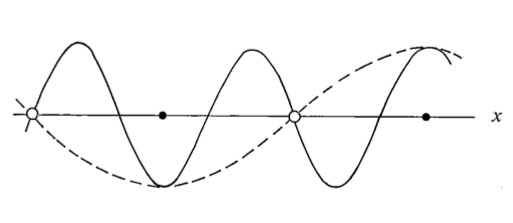
\includegraphics[width = .7 \textwidth]{figs/NM/pic61.jpg}
\caption{} \label{fig:}
\end{figure}

In a more general case, suppose that the function u consists of a number
of harmonic components

\[u = \sum_{n}^{}u_{n}\]

The nonlinear term will then contain products of harmonics of different
wave lengths, such as

\[\sin{k_1}x\sin{k_2}x\]

However,

\[\sin{k_1 x}\sin{k_2 x} = \frac{1}{2}
\left\lbrack \cos{( k_{1} - k_{2} )x - \cos{( k_{1} + k_{2} )x}} \right\rbrack\]

Thus, even if a finite difference calculation is started with waves
which all have \(k \leq k_{max}\), very soon through this process of
nonlinear interaction waves will be formed with \(k > k_{max}\) , and a
misrepresentation of waves will occur.

In general we can write

\[\sin{kx} = \sin{\left[ 2 k_{max} - ( 2 k_{max} - k ) \right] x}\]

Substituting here \(k_{max} = \frac{\pi}{\Delta x}\) and using the
formula for the sine of a difference, we obtain

\[\sin{kx} = \sin{\frac{2\pi}{\Delta x}x}\cos{\left( \frac{2\pi}{\Delta x}
- k \right)}x - \cos{\frac{2\pi}{\Delta x}x}\sin{\left( \frac{2\pi}{\Delta x} - k \right)}x\]

However, at the grid points \(x = j\Delta x\) and

\[\sin\frac{2\pi}{\Delta x}j\Delta x = 0, \qquad \cos{\frac{2\pi}{\Delta x}j\Delta x = 1}\]

Therefore, we find

\[\sin{k j \Delta x} = -\sin{\left( 2k_{max} - k \right)j\Delta x}\]

In this way, we see that, knowing only the grid point values, we cannot
distinguish the wave numbers \(k\) from \(2k_{max} - k\) . Thus, if
\(k > k_{max}\), using the convention mentioned earlier, we can say that
the wave number k is misrepresented as the wave number

\[k^{*} = 2k_{max} - k\]

Hence, as shown in \texttt{figg:62}, the resulting wave has a wave
number \(k^{*}\) which is less than \(k_{max}\) by an amount equal to
that by which \(- k\) was greater than \( k_{max}\). W e can think of
the wave number \emph{k} * as being an image obtained by the reflection
of \emph{k} across the value \(k_{max}\) into the admissible range of
wave numbers.

\begin{figure}
\centering
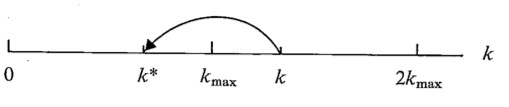
\includegraphics[width = .7 \textwidth]{figs/NM/pic62.jpg}
\caption{} \label{fig:}
\end{figure}

As an example consider the case \emph{L} = 4delta x /3, illustrated in
\texttt{figg:61}. Then \(k = 3\pi/2\Delta x\), and (6.4) gives
\(k^{*} = \frac{\pi}{2\Delta x}\) as the wave number "seen" by the
finite difference grid. This, of course, is the same wave, of wave
length \(2\Delta x\), as the one found graphically and shown by the
dashed line.

Now consider the consequences of aliasing errors in a numerical
integration. An atmospheric variable, as a function of space
co-ordinates, can be thought of as consisting of a series of harmonic
components. It is useful to consider the "energy" of these components,
that is, their contribution to the mean square value of the variable
considered as a function of wave number.

This is the \emph{spectrum} of the "energy". For example, if the
variables are velocity components, this function is the kinetic
\emph{energy spectrum}. This spectrum describes the relative importance
of features of different scales in the field of the variable. Now,
experience shows that the spectrum of atmospheric variables does not
change much with time. On synoptic maps we do not have situations where
small scale features are dominant on one day, and absent on the next.
Accordingly, spectra of atmospheric variables also do not change much in
their general shape. The energy of a particular component can, of
course, change, but the characteristic shape of the spectrum as a whole
is fairly constant. For example, a zonal spectrum of the eastward
velocity component in middle latitudes typically has a maximum for wave
numbers 4 to 7, that is, 4 to 7 wave lengths along a latitude circle,
with the energy tapering off rather rapidly as the wave number increases
beyond about 10. Thus, there is very little energy in wave numbers of
the order of the maximum wave numbers that can be resolved by finite
difference grids used in atmospheric models.

In a finite difference integration, in addition to these relatively
small physical changes, the shape of a spectrum is subject to changes
due to aliasing errors. If we have a spectrum of the shape just
described, and consider the representation of various combinations
\(k_1+k_2\) that are greater than \(k_{max}\), we see that most of the
energy of such combinations will belong to components with wave numbers
not much greater than \(k_{max}\) . Thus, due to aliasing errors a
spurious energy inflow is expected at wave numbers that are not much
less than \(k_{max}\), and, in time, the energy of these components can
be expected to grow beyond physically acceptable limits. Experience
shows that, if no precautionary measures are taken, this can indeed
happen, and even cause a catastrophic end to the integration. The
phenomenon is due to the nonlinear terms of the equations, and,
therefore, is called the \emph{nonlinear instability}. Nonlinear
instability was first encountered by Norman Phillips (1956) in his
famous work that laid the foundation for the numerical modelling of the
atmospheric general circulation. Starting from an atmosphere at rest,
he integrated the vorticity equation for a simulated time of the order
of 30 days. The calculation then came to an end due to an explosive
increase in the total energy of the system, associated with an
appearance of elongated shapes in the vorticity field. Phillips
initially believed that the breakdown was due to excessive truncation
errors, and he later repeated the experiment using space and time steps
both reduced to about half of their previous values. This must have
greatly reduced the truncation errors, but the catastrophic increase in
total energy still happened at about the same time.

In a later paper Phillips (1959) gave the interpretation of nonlinear
instability similar to what has been presented here, but for the
nondivergentvorticity equation. For a test of this explanation Phillips
again repeated his experiment, but after every two hours of simulated
time he performed a harmonic analysis of the vorticity fields, and
eliminated all components with \(k > \frac{1}{2}k_{max}\). If there are
no components with \(k > \frac{1}{2}k_{max}\) the advection term cannot
produce waves with \(k > k_{max}\) . We expect that it will be some time
before the amplitudes of the eliminated waves are built up again to an
appreciable extent. This filtering procedure eliminated the appearance
of the spurious increase in energy, thereby confirming this explanation
of the instability.

\section{Suppression and prevention of nonlinear instability}\label{sec:suppression-and-prevention-of-nonlinear-instability}

If an integration is to be performed for an extended period of time, it
is necessary to suppress or prevent nonlinear instability. For short
range integrations it is not necessary to do this, though such a
procedure might still have a beneficial effect on the model.

It has been pointed out by Orszag (1971) that to eliminate aliasing
errors it is not necessary to filter the top half of the admissible wave
numbers. It is sufficient to eliminate the top one-third, because, if
waves with \(k > \frac{2}{3}k_{max}\) are filtered out, all the aliases
satisfy \(k > \frac{2}{3}k_{max}\) and will thus be eliminated.

If, however, we consider that such a suppression of the shortest waves
is a satisfactory method of dealing with the problem, it would be
simpler to use a differencing scheme that has a built-in damping of the
shortest waves. This idea is due to Richtmyer (1963), who suggested use
of the Lax-Wendroff scheme for this purpose. It was found by experience
that such a practice does suppress the nonlinear instability, and that
to do this it is sufficient to use an intermittent Lax-Wendroff step at
quite long intervals (Kasahara, 1969). Kreiss and Oliger (1973), on the
other hand, recommend adding a dissipative term to a scheme which is not
dissipative, so that the amount of dissipation can be controlled in a
more practical way.

Another way of avoiding nonlinear instability is to use a Lagrangian
formulation of the advection terms instead of a Eulerian formulation. We
calculate the position of the parcel that should be advected to the grid
point considered in step \(\Delta t\). A value of the dependent variable
can be found corresponding to that position by interpolation in space.
The change due to advection is set equal to the difference between the
value obtained by interpolation and that at the grid point. In some
cases, these schemes turn out to be identical to schemes obtained using
the Eulerian formulation, but other schemes can also be obtained. A
procedure of this type was first used by Leith (1965); an example of its
use more recently is given in the paper by \emph{Krishnamurti et al}.
(1973).

A conceptually elegant approach for dealing with the nonlinear
instability problem has been suggested and developed by Arakawa (1966,
1972). His idea is that it is better, if possible, to use schemes for
the advection terms that are not only free of the nonlinear
computational instability but also free of the spurious inflow of
energy to these short waves, instead of artificially suppressing their
amplitudes. The amplitudes of the shortest waves in atmospheric models
are small initially, and they will remain small if a false generation of
these short waves is avoided. Arakawa has shown that it is possible to
construct such schemes, and that they are obtained when care is taken to
conserve in the finite difference form some integral properties of the
original differential equations.

When the Arakawa conservation schemes are used there is no need for an
artificial dissipation in the advection process. This enables the
statistical properties of the schemes to be maintained under advection,
a feature especially useful in general circulation studies.

It has sometimes been argued that, because the phase error of the short
waves is very large, they should be eliminated before they erroneously
affect the longer waves through nonlinear interactions.. This argument
does not take account of several factors. If the phase speeds of the
short waves are wrong, the situation will not necessarily improve if
their amplitudes are also made wrong. They may still be performing a
useful function of a statistical nature. Also damping or elimination of
the shortest waves will also remove some energy from the longer waves
that we are interested in. If we wish to dissipate energy, it is
obviously better to do so for physical and not for computational
reasons.

We shall introduce the procedure of Arakawa by considering the vorticity
equation

\[\frac{\partial\zeta}{\partial t} + \textbf{v} \cdot\nabla\zeta = 0,\qquad \zeta = \nabla^{2}\Psi\]

where the velocity \(\textbf{v}\) is assumed to be nondivergent, that is

\[\textbf{v} = \textbf{k} \times \nabla\Psi\]

Substituting this into \texttt{a7.1} we obtain

\[\frac{\partial}{\partial t}\nabla^{2}\Psi = J\left( \nabla^2\Psi, \Psi \right)\]

This equation gives the local change in vorticity as a result of
advection by a two-dimensional nondivergent velocity. It is also a
nonlinear advection equation. However, in contrast with the
one-dimensional equation \texttt{a6.1}, \texttt{a7.3} gives a good
approximate description of large scale atmospheric processes. Thus, for
more than a decade it has been used as a basic prognostic equation for
the numerical weather prediction, eventually supplemented by some
additional terms of a smaller order of magnitude.

To illustrate the Arakawa procedure for the vorticity equation (7.3), we
need some knowledge of its integral properties in wave number space. We
want to study the energy exchanges between different harmonics that are
permitted by that equation.

Consider first the kinetic energy spectrum when the velocity is
two-dimensional and nondivergent, so that it can be given by (7.2). We
can almost always assume that in the region considered A, the stream
function can be expressed as a series of orthogonal functions (e.g.
CourantandHilbert, 1953, p.369)

\[\Psi = \sum_{n}^{}\Psi_{n}\]

where the functions \(\Psi_n\) are eigenfunctions of the Helmholtz
equation

\[\nabla^{2}\Psi_{n} + \lambda_{n}^{2}\Psi_{n} = 0\]

The parameters \(\lambda_{n} \) are known as the \emph{generalized wave
numbers} of the components \(\Psi_{n}\)

As an example, let \emph{A} be a rectangular region with sides
\(L_x, L_y\). For boundary conditions assume that the stream function is
periodic in x with period \(L_{x}\) and is zero along the lower and
upper boundary. Then we can write the stream function

\[\Psi = \sum_{n_1, n_2} \left( \alpha_{n_1, n_2}\cos{\frac{2\pi n_1}{L_x}x}+
b_{n_1, n_2}\sin{\frac{2\pi n_1}{L_x}x} \right)\sin{ \frac{\pi n_2}{L_y} y}\]

Differentiating this we obtain

\[\nabla^2\Psi_n = - \left\lbrack \left( \frac{2\pi n_1}{L_x} \right)^{2} +
\left( \frac{\pi n_2}{L_y}  \right)^{2} \right\rbrack\Psi_{n}\]

that is,

\[\lambda_n^2 = \left( \frac{2\pi n_1}{L_x} \right)^{2} + \left( \frac{\pi n_2}{L_y} \right)^{2}\]

If the region \emph{A} had different geometry, another set of orthogonal
functions would satisfy \texttt{a7.5} and the boundary conditions, and
could be used for the expansion \texttt{a7.4}. These functions will be
solutions of the Helmholtz equation \texttt{a7.5}.

Define the average of a variable a by

\[\overline{\alpha} \equiv \frac{1}{A}\int_A \alpha d A\]

We are interested in the average value of the kinetic energy per unit
mass

\[\overline{K} = \frac{1}{2}\overline{( u^{2} + \nu^{2} ) } = \frac{1}{2}\overline{\nabla\Psi\cdot\nabla\Psi}\]

Substituting \texttt{a7.4}, and assuming that this series can be
differentiated and integrated term by term, we obtain

\[\overline{K} = \frac{1}{2}\overline{ \nabla \sum_n\Psi_n\cdot\nabla\sum_m \Psi_m }
= \frac{1}{2}\overline{  \sum_n\nabla\Psi_n\cdot\sum_m \nabla\Psi_m }
= \frac{1}{2}\sum_m\sum_n \overline{ \nabla\Psi_m \nabla\Psi_n }\]

We note that

\[\nabla\Psi_m \nabla\Psi_n =\nabla \cdot \left( \Psi_m\nabla\Psi_n \right) - \Psi_m\nabla^2\Psi_n\]

Assume that no mass transport occurs through the boundaries of A, that
is,

\[\overline{\nabla\cdot\left( \Psi_{m}\nabla\Psi_{n} \right)} = 0\]

Using \texttt{a7.5}, we then obtain

\[\overline{K} = -\frac{1}{2}\sum_m\sum_n \overline{ \Psi_m \nabla^2\Psi_n }
= -\frac{1}{2}\sum_m\sum_n \lambda_n^2\overline{ \Psi_m \Psi_n }\]

Since the functions \(\Psi_{n}\) are orthogonal, that is,

\[\overline{ \Psi_m \Psi_n } = 0 \qquad for m \neq n\]

the double sum reduces to a sum over only a single subscript, namely,

\[\overline{K} = \frac{1}{2}\sum_{n}\lambda_{n}^{2}\overline{\Psi_n^2}\]

We have therefore expressed the average kinetic energy in the region A
\emph{as a sum of contributions of different harmonics}

\[\overline{K} = \frac{1}{2}\sum_{n}K_n\]

Where

\[K_{n} \equiv \frac{1}{2}\lambda_{n}^{2}\overline{\Psi_n^2}\]

The contributions \(K_{n}\), considered as a function of n, represent
the kinetic energy spectrum. As seen from \texttt{a7.9}, they are never
negative. When the stream function \(\Psi\) is known, the functions
\(\Psi_{n}\) can be computed by standard series expansion methods. In
fact, we calculate the coefficients of these components; in
\texttt{a7.4}, these coefficients have been absorbed into the functions
Since the values of \(\lambda_{n}\) are already known, for commonly used
geometries, we can calculate the kinetic energy spectra using
\texttt{a7.9}. Such a calculation, as well as the calculation of the
spectra of other variables, has been used for numerous studies of the
behavior and structure of both the observed and numerically simulated
fields of atmospheric variables.

The mean square vorticity

\[\overline{\zeta^2} = \overline{(\nabla^{2}\Psi^{2} )^2}\]

can be expressed as a sum of contributions of different harmonics in a
similar way. Substituting \texttt{a7.4}, using \texttt{a7.5}, and the
orthogonality of the functions \(\Psi_{n}\), we obtain

\[\overline{\zeta^2} = \sum_{n}\lambda^{4}\overline{\Psi_n^2}\]

Substituting the expression \texttt{a7.9} for the kinetic energy of a
component \(\Psi_{n}\); we find for the average value of the enstrophy
half the vorticity squared,

\[\frac{1}{2}\overline{\zeta^{2}} = \sum_{n}\lambda_n^2 K_{n}\]

Comparing this with \texttt{a7.8} we see that the average wave number is
related to average values of enstrophy and kinetic energy. Define the
average wave number as

\[\lambda \equiv \sqrt{ \frac{\sum_n\lambda_n^2 K_n} {\sum_n K_n} }\]

Substituting (7.11) and (7.8) we find

\[\lambda = \sqrt{ \frac{\overline{\zeta_n^2} }{\overline{K}}  }\]

Thus, when the velocity is two-dimensional and nondivergent, the
average wave number is determined by the ratio of the average values of
enstrophy and kinetic energy.

We originally wished to study the time dependence of the energy of
spectral components permitted by the vorticity equation \texttt{a7.3}.
It will suffice to look at the time dependence of \texttt{a7.13}. Then
\texttt{a7.3} gives

\[\frac{\partial}{\partial t} \frac{1}{2} \overline{\zeta^2} =
\overline{\zeta \frac{\partial}{\partial t} \zeta } =
\overline{\zeta J(\zeta,\Psi)}\]

Again assuming no mass transport through the boundaries of A, we find

\[\begin{aligned}
\frac{\partial}{\partial t} \overline{K} =
\frac{\partial}{\partial t} \frac{1}{2} \overline{(\nabla\Psi)^2} =
\overline{\nabla\Psi \cdot \frac{\partial}{\partial t}\nabla\Psi} =\\
-\overline{\Psi\frac{\partial}{\partial t} \nabla^2\Psi} =
-\overline{\Psi J(\zeta,\Psi)}
\end{aligned}\]

However, for any two scalar quantities \emph{p,q} we have

\[J(p,q) = \textbf{k}\cdot\nabla \times \left( p\nabla q \right) = - \textbf{k}\nabla \times \left( p\nabla q \right)\]

Using Stokes\textquotesingle{} theorem, we see that

\[\overline{J\left( p,q \right)} = 0\]

if either \emph{p} or \emph{q} is constant along the boundary of
\emph{A}. Under the same conditions, we have

\[\overline{p J\left( p,q \right)} = 0, \qquad \overline{q J\left( p,q \right)} = 0\]

Therefore, if we assume that \(\Psi\) is constant along the boundary of
\emph{A}, \texttt{a7.14} and \texttt{a7.15} give

\[\frac{1}{2}\overline{\zeta^{2}} =  const, \quad \text{and} \quad \overline{K} = const.\]

In this way, we find that \emph{the average wave number does not change
with time} with two-dimensional nondivergent flow. In other words,
\emph{a systematic energy cascade toward higher wave numbers is not
possible}. Furthermore, since to obtain the enstrophy the contributions
\(K_{n}\) are multiplied by the wave number squared, \emph{the fraction
of the energy that can flow to high wave numbers is clearly limited, and
the higher the wave number, the more it is limited} (Fjortoft, 1953).

As pointed out by Charney (1966) this situation can be illustrated by a
simple mechanical analogy. The foregoing relations show that

\[\overline{K}\lambda^{2} = \sum_{n}K_{n}\lambda_{n}^{2} = \text{const}\]

On the left hand side here each of the two factors is constant, as the
first one is equal to the average energy. Thus, as shown in
\texttt{figg:71}, we can imagine a semi-infinite weightless rod on
which a weight \( \overline{k}\) is suspended at a distance
\(\lambda^{2}\) to the left of the point at which the rod itself is
suspended, and weights \(k_{1}k_{2}\ldots.. \) are suspended at
distances \(\lambda_{1}^{2}\lambda_{2}^{2}\ldots..\) right of that
point. The rod, as defined, would be in mechanical equilibrium. Its left
side, moreover, cannot change, while on the right hand side an
interchange of mass between weights is permitted, but only so as not to
disturb the equilibrium, that is, the total moment of forces. Thus, at
least three components must always take part in an energy transfer. In
particular very little energy can be expected to accumulate at the
highest wave numbers.

\begin{figure}
\centering
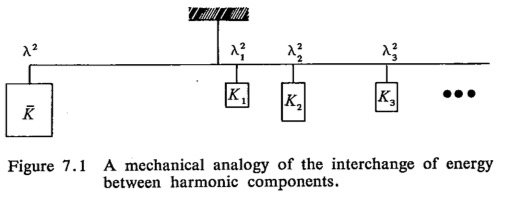
\includegraphics[width = .7 \textwidth]{figs/NM/pic71.jpg}
\caption{} \label{fig:}
\end{figure}

We now return to the numerical solution of \texttt{a7.3} and the
associated nonlinear instability problem. Obviously, if a finite
difference scheme could be constructed so as to conserve the average
values of enstrophy and the kinetic energy, the average wave number
would not change, and, therefore, a systematic transport of energy
toward the highest wave numbers would not be possible. Arakawa has
pointed this out, and showed that finite difference approximations can
be constructed that, indeed, maintain the properties \texttt{a7.17} of
the analytic Jacobian. Therefore, average enstrophy and kinetic energy
are conserved within the advection terms, and so is the average wave
number. Nonlinear instability is therefore prevented. His
approximations, in addition, maintain the property \texttt{a7.16}, and
thus also conserve the average vorticity. Thus the gross characteristics
of the frequency distribution of the vorticity field are also conserved.
The true non-divergent vorticity equation conserves all moments of the
frequency distribution of the vorticity since the area and the vorticity
of individual fluid parcels are both conserved. Maintaining properties
\texttt{a7.16} and \texttt{a7.17} in a finite difference calculation
will guarantee the conservation of the first two moments of this
distribution.

We illustrate Arakawa\textquotesingle s method by considering how to
satisfy \texttt{a7.17}. In our finite difference calculation it takes
the form

\[\overline{\zeta_{ij}J_{ij}(\zeta,\Psi)} = \frac{1}{N}\sum_{i,j}\zeta_{ij}J_{ij}(\zeta,\Psi) = 0\]

where \(J_{ij}\) denotes a finite difference approximation to the
Jacobian, and \(N\) the total number of grid points.

There are many ways of constructing finite difference approximations to
the Jacobian. We can use any of the three equivalent analytic
expressions

\[\begin{aligned}
J(p,q) = \frac{\partial p}{\partial x}\frac{\partial q}{\partial y} -
\frac{\partial p}{\partial y}\frac{\partial q}{\partial x} =\\
\frac{\partial }{\partial y}q\frac{\partial p}{\partial x} -
\frac{\partial }{\partial x}q\frac{\partial q}{\partial x} =\\
\frac{\partial }{\partial x}p\frac{\partial q}{\partial y} -
\frac{\partial }{\partial y}p\frac{\partial q}{\partial x}
\end{aligned}\]

We shall consider only approximations of the second order of accuracy.
With the simplest centered space differencing, we require values of
\(p\), \(q\) from a box of nine adjacent grid points to evaluate (7.20),
as shown in \texttt{figg:72}. Write \emph{d} for the grid size, and
\(p_{k}\), \(q_{k}\) for the values of \( p \), \(q\) at the point
denoted by \(k\). We then obtain the following approximations to the
expressions \texttt{a7.2}

\begin{figure}
\centering
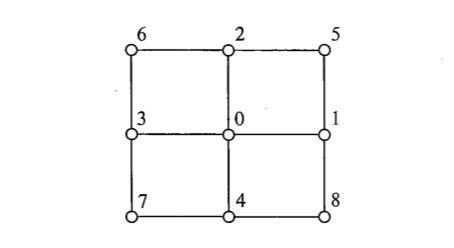
\includegraphics[width = .7 \textwidth]{figs/NM/pic72.jpg}
\caption{Stencil used to define approximations to Jacobian.}
\end{figure}

\[J^{++}(p,q) = \frac{1}{4d^2} \left[ (p_1 - p_3)(q_2 - q_4) - (p_2-p_4)(q_1-q_3) \right]\]

\[J^{\times +}(p,q) = \frac{1}{4d^2} \left[ q_2(p_5 - p_6) - q_4(p_8-p_7)
-q_1(p_5 - p_8) - q_3(p_6-p_7)  \right]\]

\[J^{+ \times}(p,q) = \frac{1}{4d^2} \left[ p_1(q_5 - q_8) - p_3(q_6 - q_7)
- p_2(q_5 - q_6) - p_4(q_8 - q_7)  \right]\]

The superscripts \(+\) and \(\times\) denote the positions of the points
from which values of \(p\) and \(q\), respectively, are used to form the
approximation. Each of the approximations \texttt{a7.21a},
\texttt{a7.21b}, \texttt{a7.21c} is consistent and of the second order
of accuracy. A more general approximation can now be formed as a linear
combination of these three, that is

\[J(p.q) = \alpha J^{++} + \beta J^{\times +} + \gamma J^{+\times}\]

With the consistency requirement

..math:: alpha + beta + gamma = 1

This approximation is also of the second order of accuracy.

When evaluating the sum in \texttt{a7.19} using \texttt{a7.22} we obtain
24 terms from each grid point in the computational region. All of these
terms will be of the form
\(\text{const} \cdot\zeta_{k}\zeta_{l}\Psi_{m}\). By choosing the
constants \(d,\beta,\gamma\) appropriately we can make all of these
terms cancel out in the summation process, thereby fulfilling
\texttt{a7.19}. For example, the point \emph{0} will contribute terms to
\texttt{a7.19} of the form

\[\zeta_0 J_0( \zeta,\Psi ) = \frac{1}{4d^{2}}\left( \alpha \zeta_{0} \zeta_{1}\Psi_{2} \right)
\quad + \quad \text{23 more terms}\]

A term containing \(\zeta_{0}\zeta_{1}\Psi_{2}\) will also appear in the
expression for \(\zeta_{1}J_{1}\left( \zeta,\Psi \right)\). Because of
the form of the Jacobian approximations \texttt{a7.21a} it will have to
come from the product \(p_{3}q_{6}\). Thus, one contribution from the
point 1 will be

\[\alpha = \beta = \gamma = \frac{1}{3}\]

These two terms will cancel if \(\alpha = \beta\) . Arakawa has shown
that, when

\[\zeta_{1}J_{1}\left( \zeta,\Psi \right) = \frac{1}{4d^{2}}\left( \ldots\beta\zeta_{1}\zeta_{0}\Psi_{2} + \ldots \right).\]

not only do all the terms in the sum \texttt{a7.19} cancel, but also all
the terms in the expression for the conservation of the average kinetic
energy, and the average vorticity (Arakawa, 1966; Lilly, 1965). Thus,
the approximation

\[J_{A} \equiv \frac{1}{3}\left( J^{+ +} + J^{\times +} + J^{+ \times} \right)\]

will conserve average vorticity, enstrophy and kinetic energy when used
for the numerical solution of \texttt{a7.3}. This is more than
sufficient for the prevention of nonlinear instability. The
approximation \texttt{a7.23} is usually called the \emph{Arakawa
Jacobian}. Arakawa has also shown how to construct an approximation of
fourth order accuracy to the Jacobian, conserving these three
quantities.

It has recently been demonstrated (Jespersen, 1974) that the Arakawa
Jacobian can be derived as a special case of the so called "finite
element method", a relatively new and promising development in the field
of the numerical solution of partial differential equations. Instead of
approximating the space derivatives by finite differences, the finite
element method consists of using an interpolation procedure to convert a
set of values given at grid points into a field given everywhere. This
is done using a variational formulation, minimizing the error of the
approximation (e.g. Cullen, 1974).

Arakawa has constructed an analogue of the scheme \texttt{a7.23} for the
vorticity equation to approximate the advection terms in the primitive
equations in the case when the wind is nondivergent. This scheme is then
generalized to allow for divergence (Arakawa, 1972; Arakawa and Lamb,
1976).

In conclusion, we stress that the essence of the Arakawa method is to
control the computational energy cascade, by conservation of the average
wave number within the advection terms due to the nondivergent part of
the flow.

Thus, it is not only a conservation of energy, as has sometimes
incorrectly been implied. For example, an approximation can easily be
constructed for the nonlinear term of the one-dimensional advection
equation \texttt{a6.1} which would conserve the kinetic energy. Using
such an approximation, however, would not prevent nonlinears instability
in the way that the Arakawa scheme does. The Arakawa procedure does not
have a one-dimensional analogue, as the nondivergentvorticity equation
\texttt{a7.3} is not nonlinear when applied to a one-dimensional
problem.